\chapter{Toisen luvun otsikko} \label{Toinen luku}

Tässä luvussa tarkastellaan kahden kuvan upottamista samaan kelluvaan
kuvaympäristöön (Kuva \ref{fig:Optimointia-kahdella-eri}).

\begin{figure}[tbh]
\subfloat[Käynnistysajan optimointi Nailgunilla.]{\begin{centering}
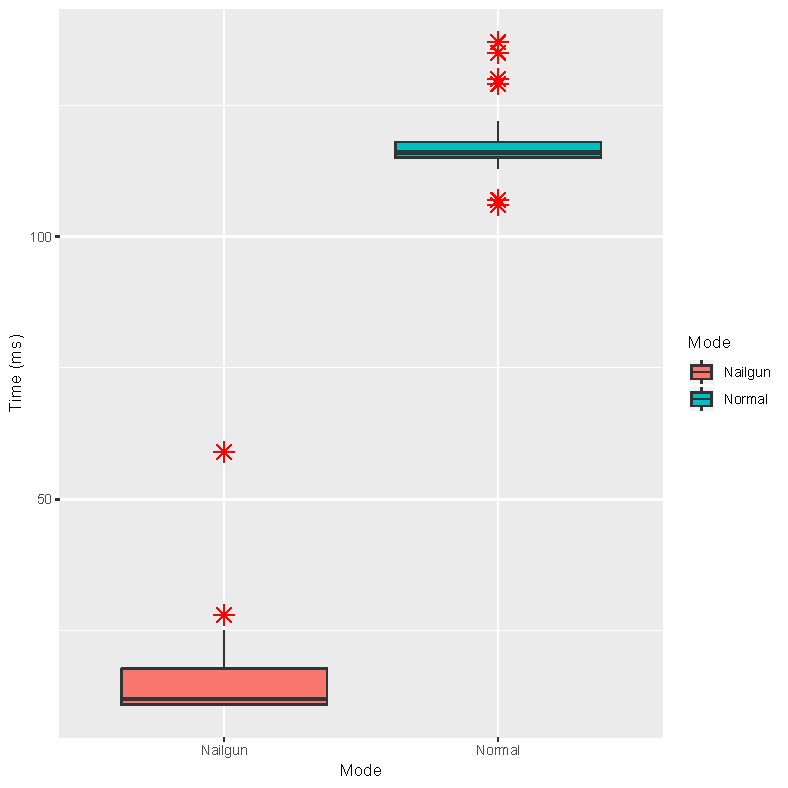
\includegraphics[width=0.45\textwidth]{kuvat/nailgun.pdf}
\par\end{centering}
}\subfloat[Koon optimointi Proguardilla.]{\begin{centering}
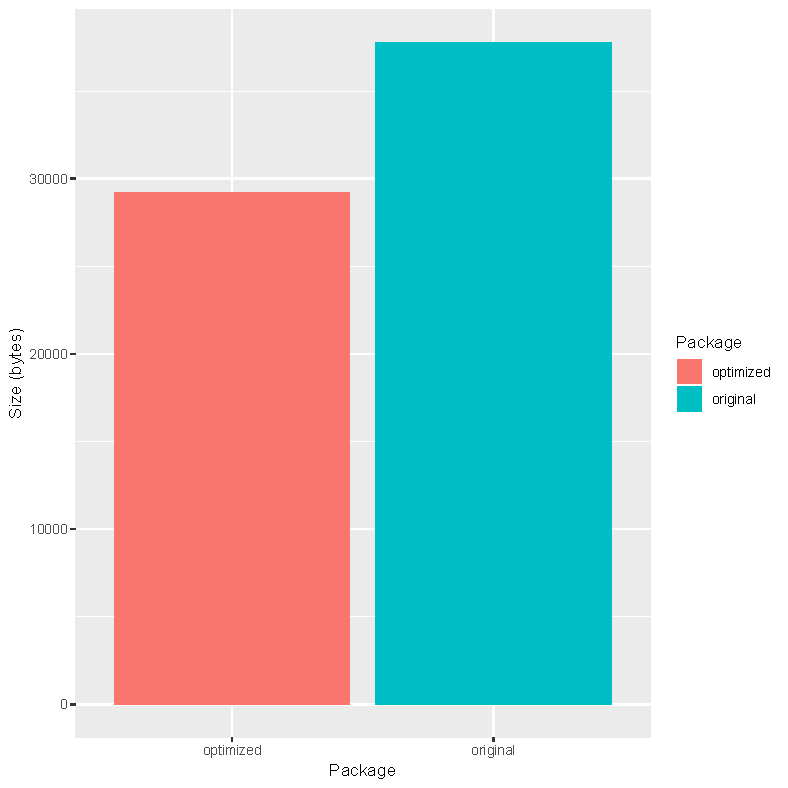
\includegraphics[width=0.45\textwidth]{kuvat/proguard.pdf}
\par\end{centering}
}\caption{Optimointia kahdella eri tavalla.\label{fig:Optimointia-kahdella-eri}}

\end{figure}

